\documentclass[preprint,12pt]{elsarticle}
\usepackage{amsmath}
\usepackage{amsfonts} %potrzebne do \mathbb{S}
\usepackage{here}
\usepackage{caption}
\usepackage{subcaption}
\usepackage{color}
\def\spe{\mathbf{Spec}}
\usepackage{graphicx}
\usepackage{soul}           %package for highlight
\newcommand{\noop}[1]{}
\newtheorem{problem}{Problem}
\usepackage{lineno,hyperref}
\modulolinenumbers[5]
\journal{Mechanical Systems and Signal Processing}


%% `Elsevier LaTeX' style
%\bibliographystyle{abbrvnat}%\biboptions{sort&compress}
\bibliographystyle{elsarticle-num}\biboptions{sort&compress}
%%%%%%%%%%%%%%%%%%%%%%%

\begin{document}

\begin{frontmatter}

\title{Optimal filter design with progressive genetic algorithm for local damage detection in rolling bearings}


%% Group authors per affiliation:
\author[label1]{Jacek Wodecki \corref{cor1}}
\cortext[cor1]{Corresponding author, jacek.wodecki@pwr.edu.pl}
\author[label2]{Anna Michalak}
\author[label1]{Radoslaw Zimroz}

\address[label1]{Diagnostics and Vibro-Acoustic Science Laboratory, Wroclaw University of Science and Technology, Na Grobli 15, 50-421 Wroclaw
\\\{jacek.wodecki, radoslaw.zimroz\}@pwr.edu.pl\\}
\address[label2]{KGHM Cuprum Ltd, Research and Development Centre, Sikorskiego 2-8, 53-659 Wroclaw, Poland
\\ amichalak@cuprum.wroc.pl\\}

\begin{abstract}
Harsh industrial conditions present in underground mining cause a lot of difficulties for local damage detection in heavy-duty machinery. For vibration signals one of the most intuitive approaches of obtaining signal with expected properties, such as clearly visible informative features, is prefiltration with appropriately prepared filter. Design of such filter is very broad field of research on its own. In this paper authors propose a novel approach to dedicated optimal filter design using progressive genetic algorithm. Presented method is fully data-driven and requires no prior knowledge of the signal. It has been tested against a set of real and simulated data. Effectiveness of operation has been proven for both healthy and damaged case. Termination criterion for evolution process was developed, and diagnostic decision making feature has been proposed for final result determinance.
\end{abstract}

\begin{keyword}
local damage, vibration, genetic algorithm, digital filter
\end{keyword}

\end{frontmatter}

\linenumbers

\section{Introduction}

In the field of machine diagnostics based on vibration signal analysis, information about the damage is placed in so called informative frequency band (IFB) \cite{obuchowski2014selection}. Span of this band depends on many factors, such as kinematic structure, operational conditions, type of damage and its location within the machine. In other words: it depends on design, operational, change of conditions factors as was stated by Bartelmus \cite{bartelmus2009new}. In most cases neither those factors nor information about IFB are known. Facing such limitations, it is clear that pursuit for automatic, data-driven methods is the most desirable direction of research. Many different techniques for IFB identification have been developed over the years, such as adaptive wavelet-based filtration \cite{nikolaou2002demodulation,peter2004machine}, filtering with spectral kurtosis \cite{antoni2009cyclostationarity,antoni2006spectral}, modulation intensity distribution \cite{urbanek2012detection}, empirical mode decomposition \cite{flandrin2004empirical,liu2006gearbox,lei2013review}, selectors \cite{obuchowski2014recent,wylomanska2016impulsive,zak20161932}, protrugram \cite{barszcz2011novel}, sparsogram \cite{peter2013design,peter2013automatic} or stochastic resonance \cite{lei2013planetary}.

In presented solution authors pursue the approach of determining IFB, and hence extracting information about the presence of damage, that is based on optimal filtration. In opposition to using classic adaptive filters \cite{makowski2014new,makowski2013procedure} or designing optimal filter prior to predefined specification \cite{nilsson2003digital}, presented approach is fully data-driven, and fitness function evaluates the solutions only in terms of filtration performance. This way no functional constraints are imposed on the way that filter is constructed by the evolution process. Real-life data utilized in this paper were previously addressed in \cite{wodecki2017local}.

From mathematical point of view, filter is just an equation of discrete transfer function with N coefficients. For optimal filtering, both the value of N and coefficients values should be found. From such perspective, diagnostic methodology can be considered as multidimensional optimization problem. Genetic Algorithm (GA) is one of the most frequently used tool for that task. However, it should be noted that presented procedure is not a simple application of GA to filter design. Authors proposed a complete progressive procedure for data-driven arbitrary filter development having no prior requirements. Kurtosis of filtered signal is used as a fitness function, since local damage in rotating machines presents itself as wideband impulses in vibration signal. However, an original concept of termination procedure is proposed. In this paper, progressive genetic algorithm has been applied for the design of linear phase digital FIR filter. Presented method is compared with filtration based on spectral kurtosis (SK) and kurtogram, which are selected as the classical methods of custom filtration.


\section{Methodology}
\subsection{Genetic Algorithm}
In computer science and operations research, a genetic algorithm (GA) is a metaheuristic inspired by the process of natural selection that belongs to the larger class of evolutionary algorithms (EA) \cite{darwin2008origin}. Genetic algorithms are commonly used to generate high-quality solutions to optimization and search problems by relying on bio-inspired operators such as mutation, crossover and selection \cite{mitchell1998introduction}. This idea appeared first in 1967 in J. D. Bagley’s thesis “The Behavior of Adaptive Systems Which Employ Genetic and Correlative Algorithms” \cite{bagley1967behavior}. The theory and applicability was then strongly influenced by J. H. Holland, who can be considered as the pioneer of genetic algorithms \cite{holland1992adaptation,holland1989induction}. Since then, this field has witnessed a tremendous development.

% Let us restrict to the view that genetic algorithms are optimization methods. In general, optimization problems are given in the following form:

% \begin{problem}
% Find an $x_0\in \mathbf{X}$ such that f is maximal in $x_0$, where $f:\mathbf{X}\rightarrow \mathbb{R}$ 
% is an arbitrary real-valued function, i.e. 
% \begin{equation}
% \label{eq:problem1}
% f(x_0)=\max_{x\in X}⁡f(x_0)
% \end{equation}
% \end{problem}

% In practice, it is sometimes almost impossible to obtain global solutions in the strict sense of (\ref{eq:problem1}). Depending on the actual problem, it can be sufficient to have a local maximum or to be at least close to a local or global maximum. So, let us assume in the following that we are interested in values \emph{x} where the value of objective function \emph{f} is maximized.
% The search space \textbf{X} can be seen in direct analogy to the set of competing individuals in the real world, where \emph{f} is the function which assigns a value of “fitness” to each individual (this is, of course, a serious simplification).
% The following table gives a list of different expressions, which are common in genetics, along with their equivalent in the framework of GAs:
% \begin{table}[ht!]
%     \centering
%     \caption{Naming relations between natural evolution and genetic algorithm}
%     \begin{tabular}{|l|l|}
%     \hline
%          Natural Evolution & Genetic Algorithm \\ \hline
%          Genotype & Coded string \\
%          Phenotype & Uncoded string \\
%          Chromosome & String \\
%          Gene & String position \\
%          Allele & Value at a certain position \\
%          Fitness & Objective function value \\
%     \hline
%     \end{tabular}
%     \label{tab:tab1}
% \end{table}

% After this preparatory work, the b

Basic structure of a genetic algorithm presents itself as follows (see Fig. \ref{fig:block}).

\begin{figure}[ht!]
\centering
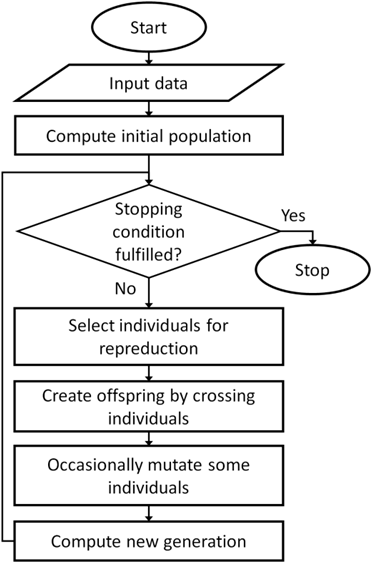
\includegraphics[width=0.48\textwidth]{wykresy/block.png}
\caption{Functional flowchart of genetic algorithm}
\label{fig:block}
\end{figure}

As obvious from the above algorithm, the transition from one generation to the next consists of four basic components \cite{mitchell1998introduction}:

\begin{itemize}
    \item \textbf{Selection:} Mechanism for selecting individuals (strings) for reproduction according to their fitness (objective function value).
    \item \textbf{Crossover:} Method of merging the genetic information of two individuals; if the coding is chosen properly, two good parents produce good children.
    \item \textbf{Mutation:} In real evolution, the genetic material can by changed randomly by erroneous reproduction or other deformations of genes, e.g. by gamma radiation. In genetic algorithms, mutation can be realized as a random deformation of the strings with a certain probability. The positive effect is preservation of genetic diversity and, as an effect, that local maxima can be avoided.
    \item \textbf{Sampling:} Procedure which computes a new generation from the previous one and its offspring.
\end{itemize}

Compared with traditional continuous optimization methods, such as Newton, quasi-Newton or gradient descent methods, we can state the following significant differences \cite{fletcher2013practical}:

\begin{enumerate}
    \item While almost all conventional methods search from a single point, GAs always operate on a whole population of points (strings). This contributes much to the robustness of genetic algorithms. It improves the chance of reaching the global optimum and, vice versa, reduces the risk of becoming trapped in a local stationary point.
    \item Normal genetic algorithms do not use any auxiliary information about the objective function value such as derivatives. Therefore, they can be applied to any kind of continuous or discrete optimization problem. The only thing to be done is to specify a meaningful decoding function. 
    \item GAs use probabilistic transition operators while conventional methods for continuous optimization apply deterministic transition operators. More specifically, the way a new generation is computed from the actual one has some random components.
\end{enumerate}

\subsection{Filter encoding}

Filter is a frequency selective object that allows a certain frequency to pass while attenuating the others. Traditionally, different techniques exist for the design of digital filters. Of these, windowing method is the most popular \cite{oppenheim1999discrete}. In this method, ideal impulse response is multiplied with a window function. There are various kinds of window functions (Butterworth, Chebyshev, Kaiser etc.), depending on the requirements of ripples on the passband and stopband, stopband attenuation and the transition width. These various windows limit the infinite length impulse response of ideal filter into a finite window to design an actual response. But windowing methods do not allow sufficient control of the frequency response in the various frequency bands and other filter parameters such as transition width. Designer always has to compromise on one or the other of the design specifications. So, evolutionary methods have been implemented in the design of digital filters to design with better parameter control. Since population based stochastic search methods have proven to be effective in multidimensional nonlinear environment, all of the constraints of filter design can be effectively taken care of by the use of these algorithms. 
Consider digital FIR filter with the following transfer function:

\begin{equation}
\label{eq:fir}
\frac{x_n}{y_n}=a_0 + a_1 z^{-1} + a_2 z^{-2} +\dots +a_n z^{-n}
\end{equation}
where $\{a_1,\dots ,a_n \}$ are values of the filter coefficient vector. Since linear phase within the passbands of the filter is desired, authors decided to use symmetric coefficient vector with odd number of coefficients. Such approach can also allow to optimize the execution time since only one half of the coefficients has to be evolved. The GA encoding of a filter is a string (chromosome), containing half of the coefficient vector $A=\{a_l,a_{l+1},a_{l+2},\dots,a_n\}$, where $a_l$ is the middle coefficient. The search space for such real-value encoding is defined as:

\begin{equation}
\label{eq:ar}
A\in \mathbb{R}
\end{equation}

Since FIR filters are inherently stable, there is no need to impose any search space constraints regarding zeros or poles on the \emph{Z} plane.

\subsection{Fitness function}

Different kinds of fitness function can be used for this kind of problem \cite{mitchell1998introduction}. Various approaches have been investigated, and they can be divided into two main categories:

\begin{itemize}
    \item Investigation of cyclicity / periodicity, e.g. sample coherence, Fourier-based measures,
    \item Investigation of impulsiveness / distance from Gaussian distribution, e.g. heavy-tailed parameters, simple statistics.
\end{itemize}

In this particular application authors follow the second approach and ordinary kurtosis was used as defined below:

\begin{equation}
\label{eq:kurtosis}
Kurt[X]=\frac{m_4}{{m_2}^2}=\frac{\frac{1}{n} \sum_{i=1}^{n} \left(x_i - \overline{x} \right)^4}{\left({\frac{1}{n} \sum_{i=1}^{n} \left(x_i - \overline{x} \right)^2}\right)^2}
\end{equation}
where $m_4$ is the fourth central moment and $m_2$ is the second sample moment (sample variance).

It is not very hard to justify the usage of kurtosis. In case of rotating machines, local damage reveals itself in vibration signal as wideband, typically periodic impulses. Since they cover wide range of frequency spectrum, they are expected to be short and sharp. It can be anticipated that kurtosis will be very susceptible to those as a fitness function.

Fitness value plays the role of  the operator used by algorithm itself, however for visual inspection of obtained IFB influencing the signal structure, spectrogram is used. It is calculated as a square of absolute values of the short-time Fourier transform (STFT). The STFT for the discrete signal x[0], x[1], \dots , x[N-1] is defined as follows \cite{oppenheim1999discrete}:

\begin{equation}
\label{eq:spectrogram}
STFT(n,k)=\sum_{m=0}^{L-1} x[n+m]\omega[m]e^{-j2\pi km/N}
\end{equation}
for $0\leq k\leq N-1$. In the above equation $\omega[.]$ is the shifted window of the length L.

\subsection{Progressive GA} \label{pga}

The concept of progressiveness of genetic algorithm realizes the idea of application robustness.  Let us assume that GA evolves whole, relatively long chromosome for a given individual, right from the beginning. This approach is susceptible to misdirected evolution. Since in our application filter coefficients are evolved, long chromosome translates into large number of coefficients, and this means that filter would be able to come out with relatively high precision. Since the coefficients’ vector is randomly initiated, high-precision filter evolution very often goes the wrong way, and despite fulfilling the condition of increasing value of the fitness function, it can be lead to local maximum, which is not always easy to be fixed by random mutation. 

To avoid this effect, authors propose to start with short chromosome and increase its length every epoch that lasts predefined amount of generations (of course unless it will be terminated by stall limit constraint). It is realized by starting with short, very general filter at the beginning. First epoch is expected to optimize this filter, and since it is short, it will capture the general shape of filter response, towards which the evolution should proceed. Consecutive epochs extend the previously optimized coefficients’ vector by two additional random entries for each individual. This way filter precision gradually increases, with general direction of evolution being preserved by shorter filter optimized in previous epoch.
Extensive testing shows that such approach results in faster, more effective evolution. Utilization of well known test data to be filtered proved, that local maxima are successfully avoided every time, which is hardly ever the case with evolving the whole filter at once.

\subsection{Termination criterion}

Hence PGA is characterized with several types of irregular behavior such as previously described stepped fitness progression or negative peaks, it is not easy to use any trivial, commonly used termination criteria like derivative of fitness progression. To deal with such complex behavior, it is proposed to use normalized root mean square error (NRMSE) between fitness progression within a single epoch, and its linear approximation. Error is normalized to statistic span of the fitness progression vector up to given point, and its threshold is set at $5\%$:

\begin{equation}
\label{eq:spectrogram}
NRMSE(y_k,\hat{y_k})=\frac{1}{y(end) - y(1)}\sqrt{\frac{\sum_{i=1}^{n} \left(y_k - \hat{y_k} \right)^2}{n}}
\end{equation}
where $y_k$  is the fitness function segment of $k^{th}$ epoch, $\hat{y_k}$ ̂is its linear fit obtained by ordinary linear regression, $y(1)$ is first value of entire fitness vector, $y(end)$ is the current last value of fitness vector, and \emph{n} is the length of regarded segment.


\subsection{Signal simulation for reference scenarios} \label{sim}

In simulated data authors intended to preserve overall structure of the signal, but with possibility to precisely control behavior of the impulses (see Fig. \ref{fig:block2}). As a first step, impulse response of the mechanical system of the bearing inside the pulley has been captured using Autoregressive Moving Average model (ARMA) that was estimated for the real signal \cite{brockwell2013time}. It has been shown that such model is appropriate for modeling healthy vibration signal \cite{pham2010estimation}. It was then convolved with the excitation signal, which is the comb of 10 Hz impulses with just a little additive white Gaussian noise to preserve simulated signal from taking values of zero between impulse events. Amplitudes of the impulses were not all equal, but also randomized with Gaussian noise. 

\begin{figure}[ht!]
\centering
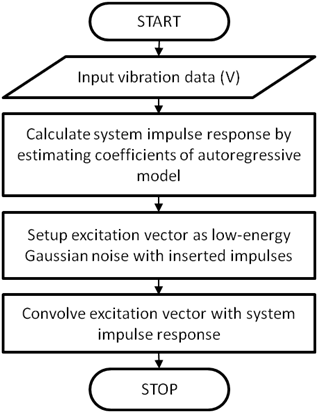
\includegraphics[width=0.48\textwidth]{wykresy/block2.png}
\caption{Simulation procedure flowchart}
\label{fig:block2}
\end{figure}

Signal was prepared in a way that it would not be easier to process than the real one. Average energy of the impulses was adjusted so that they are barely visible but not very obvious in the time series. In case of simulating healthy component, impulses were omitted and excitation signal was just a noise, which allowed to obtain only the spectral structure of the signal from healthy machine.

\section{Application to industrial data}

In this section the application of described methodology to real and simulated data is presented. Authors evaluate performance of the algorithm using simulate data describing healthy and damaged bearing, and finally using real-life data from damaged bearing. Parameters of designed real-coded progressive genetic algorithm (PGA) are presented in Table \ref{tab:tab2}.

\begin{table}[ht!]
    \centering
    \caption{Parameters of PGA}
    \begin{tabular}{|l|l|}
    \hline
         \textbf{Parameter} & \textbf{Value} \\ \hline
         Initial filter length & 7 \\ \hline
         Population size & 150 \\ \hline
         Termination criterion & NRMSE \\ \hline
         Generations per epoch & 80 \\ \hline
         Initial population & Random $\sim$ N(0,1) \\ \hline
         Selection & Roulette \\ \hline
         Crossover & Heuristic with d=1.5 \\ \hline
         Mutation & Uniform with R=0.01 \\ \hline
         Stall limit & 20 \\ \hline
         Average change for stall limit & $10^{-6}$ \\ \hline
         Elite individuals & 3 \\
    \hline
    \end{tabular}
    \label{tab:tab2}
\end{table}

\subsection{Reference case 1 - simulated signal of healthy bearing} \label{rc1}

To verify algorithms performance two reference scenarios have been tested. First of them is the case of testing the algorithm against the possibility of false-positive information occurrence with simulated signal describing healthy bearing. Signal has been prepared according to the description in section \ref{sim} omitting the impulses (Fig. \ref{fig:simh1} a, c), and its envelope spectrum corresponds to general spectral structure of mechanical systems impulse response (Fig. \ref{fig:simh1} b). Kurtosis of simulated signal is equal to 3.03 and after processing it increases only to 3.07 (only about 1$\%$ improvement), which can indicate of lack of local damage. Processing with designed filter produced signal almost identical in terms of its envelope spectrum, and the only significant change in the spectral structure is bringing down low-frequency high-energy frequency band that can be observed as change in scale of the energy axis (Fig. \ref{fig:simh1} e, f). 

\begin{figure}[ht!]
\centering
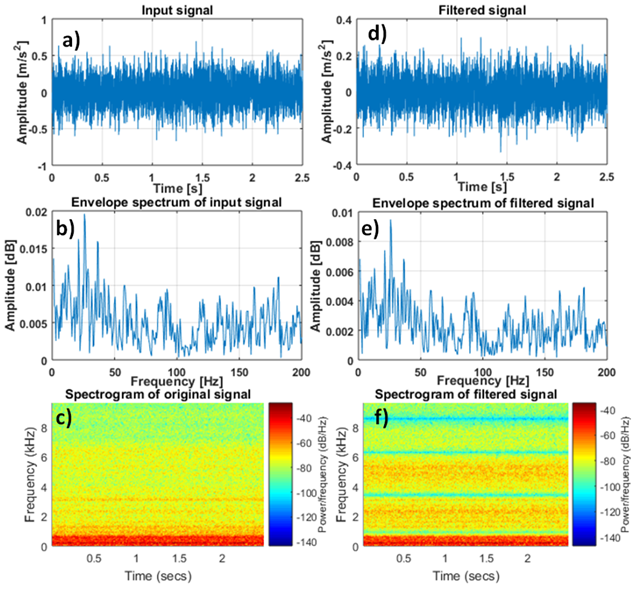
\includegraphics[width=0.8\textwidth]{wykresy/simh1.png}
\caption{Comparison between simulated input and output signals describing healthy machine. a) time series of input signal, d) time series of filtered signal, b) envelope spectrum of input signal, e) envelope spectrum of output signal overlaying the original one, c) spectrogram of input signal, f) spectrogram of output signal}
\label{fig:simh1}
\end{figure}

Coefficient vector does not reveal any particular behavior (Fig. \ref{fig:simh2} a). One can see that fitness progression reveals different character than for the signal containing damage, because there is no noticable transition from first to second stage, hence no critical length point can be observed (Fig. \ref{fig:simh2} b). Magnitude response function is rather arbitrary and does not present any convincing IFB structure (Fig. \ref{fig:simh2} c). Termination function values are presented in Fig. \ref{fig:simh3}. Final value that algorithm terminates at, is equal to 4.84.

\begin{figure}[ht!]
\centering
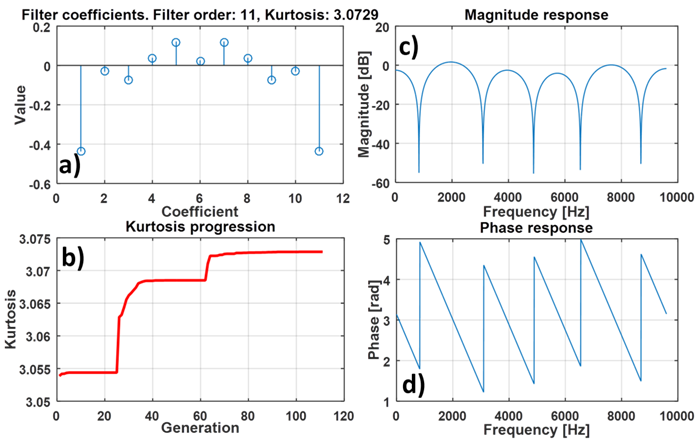
\includegraphics[width=0.8\textwidth]{wykresy/simh2.png}
\caption{Final results of filter optimization for simulated healthy case: a) vector of filter coefficients, b) fitness progression, c) magnitude response of obtained filter, d) phase response of obtained filter}
\label{fig:simh2}
\end{figure}

\begin{figure}[ht!]
\centering
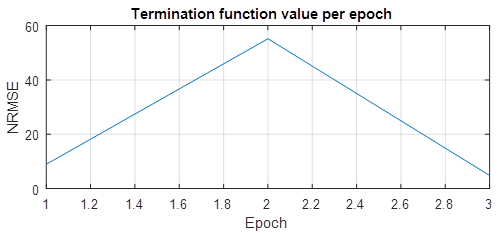
\includegraphics[width=0.7\textwidth]{wykresy/simh3.png}
\caption{Values of termination function for simulated healthy signal}
\label{fig:simh3}
\end{figure}

\subsection{Reference case 2 - simulated signal of damaged bearing}

Second reference scenario concerns processing simulated signal of damaged bearing. Signal has been prepared in specific way, as a mixture of pure damage component and healthy component prepared as for section \ref{rc1} (Fig. \ref{fig:simd1} a, b). Component of damage has been simulated similarly, but this time excitation vector contains strong impulses and very low level of noise. Combination of those two components produces input signal for the algorithm (Fig. \ref{fig:simd1} c). It is important to recognize the difference between the envelope spectra (Fig. \ref{fig:simd1} d, e) and spectrograms of the components (Fig. \ref{fig:simd1} g, h), and see how their spectral structure combines into the input signal (Fig. \ref{fig:simd1} f, i). Kurtosis value of simulated signal equal to 3.35 does not clearly inform about any sign of impulsiveness in the data. 

\begin{figure}[ht!]
\centering
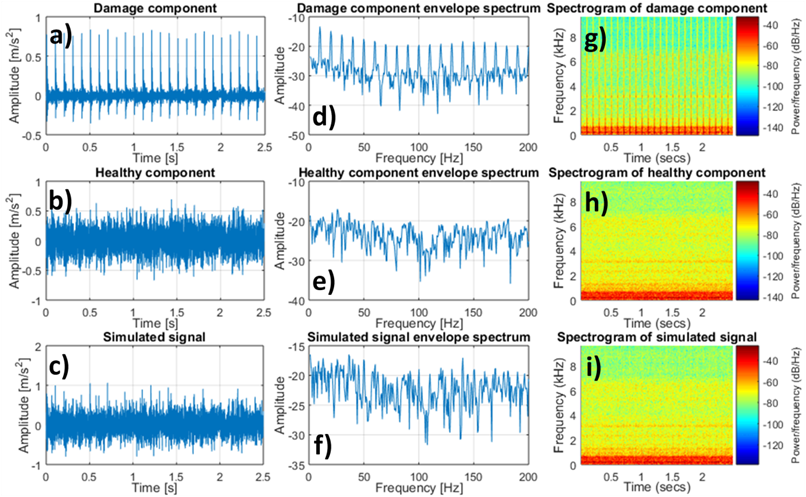
\includegraphics[width=1\textwidth]{wykresy/simd1.png}
\caption{Scenario of damage signal simulation. Signals: a) damage component, b) healthy component, c) combined components. Envelope spectra of: d) damage component, e) healthy component, f) combined components. Spectrograms of: g) damage component, h) healthy component, i) combined components}
\label{fig:simd1}
\end{figure}

Results of the algorithm operation turned out to be very successful. Kurtosis of output signal was equal to 15.03 (improvement ratio of 348$\%$). Filtered signal reveals clear and sharp impulses that undoubtedly inform about the presence of local damage (Fig. \ref{fig:simd2} d). Envelope spectrum of filtered signal differs significantly from the original one, revealing series of harmonic frequencies related to impulsive behavior (Fig. \ref{fig:simd2} b, e). In case of healthy signal simulation there was no impulsiveness to be found, so discovered IFB was expected to be flat or not clearly defined. In case of local damage simulation, introduced impulses were very narrow, which resulted in occupying whole frequency range. Because of that, IFB is broader, and beside minor modifications in the full frequency range, the most important spectral effect is the suppression of very energetic low frequencies, which is the main factor of successful filtration of such signal (Fig. \ref{fig:simd2} e, f).

\begin{figure}[ht!]
\centering
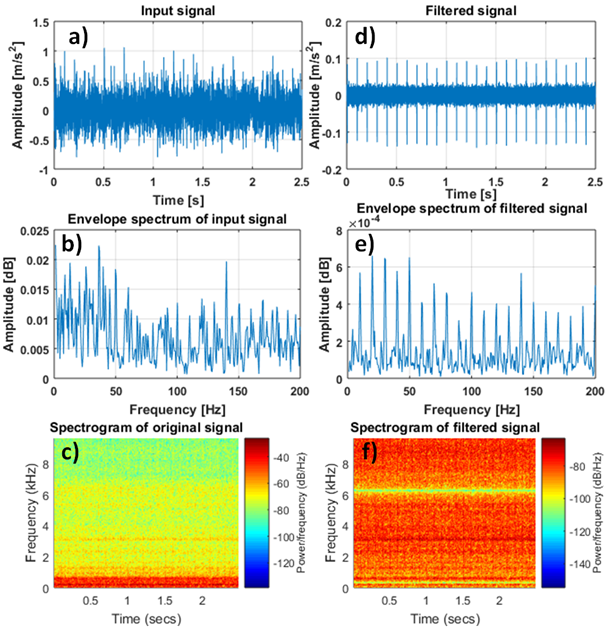
\includegraphics[width=0.8\textwidth]{wykresy/simd2.png}
\caption{Comparison between input and output signals. a) time series of input signal, d) time series of filtered signal, b) envelope spectrum of input signal, e) envelope spectrum of output signal overlaying the original one, c) spectrogram of input signal, f) spectrogram of output signal}
\label{fig:simd2}
\end{figure}

As explained before, IFB is very broad and relatively even regarding attenuation within passbands (Fig. \ref{fig:simd3} c). Fitness progression contains a lot of negative peaks (Fig. \ref{fig:simd3} b). It is a great example illustrating that extending well-established filter by additional random coefficients can cause massive reduction of its quality. For this signal, point of critical length occurs very early – in the first epoch. It means that in some cases evolution does not need much time to produce general structure of the filter, that already behaves relatively well. Termination function values are presented in Fig. \ref{fig:simd4}. Final value that algorithm terminates at, is equal to 0.54.

\begin{figure}[ht!]
\centering
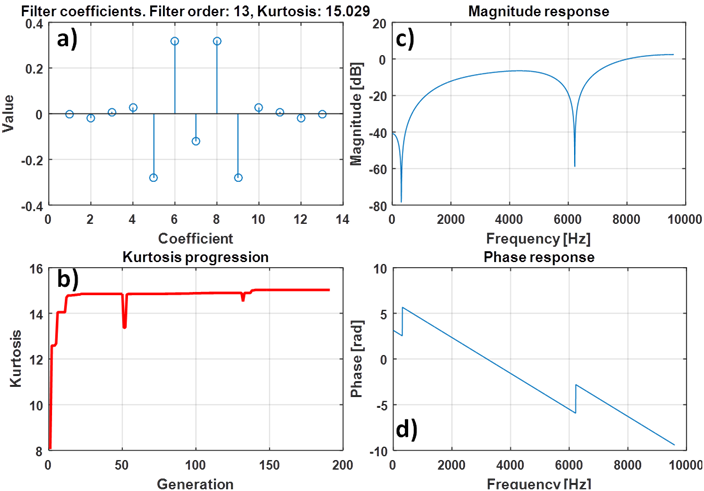
\includegraphics[width=0.85\textwidth]{wykresy/simd3.png}
\caption{Results of filter optimization: a) vector of filter coefficients, b) fitness progression, c) magnitude response of obtained filter, d) phase response of obtained filter}
\label{fig:simd3}
\end{figure}

\begin{figure}[ht!]
\centering
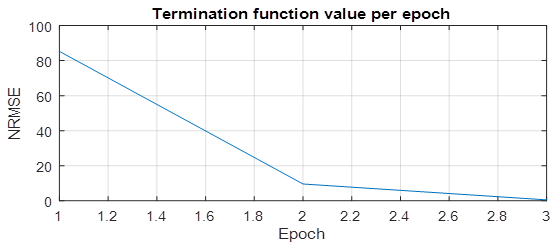
\includegraphics[width=0.7\textwidth]{wykresy/simd4.png}
\caption{Values of termination fuction for simulated damage signal}
\label{fig:simd4}
\end{figure}

\subsection{Real-life data - raw vibration signal}

\begin{figure}[ht!]
\centering
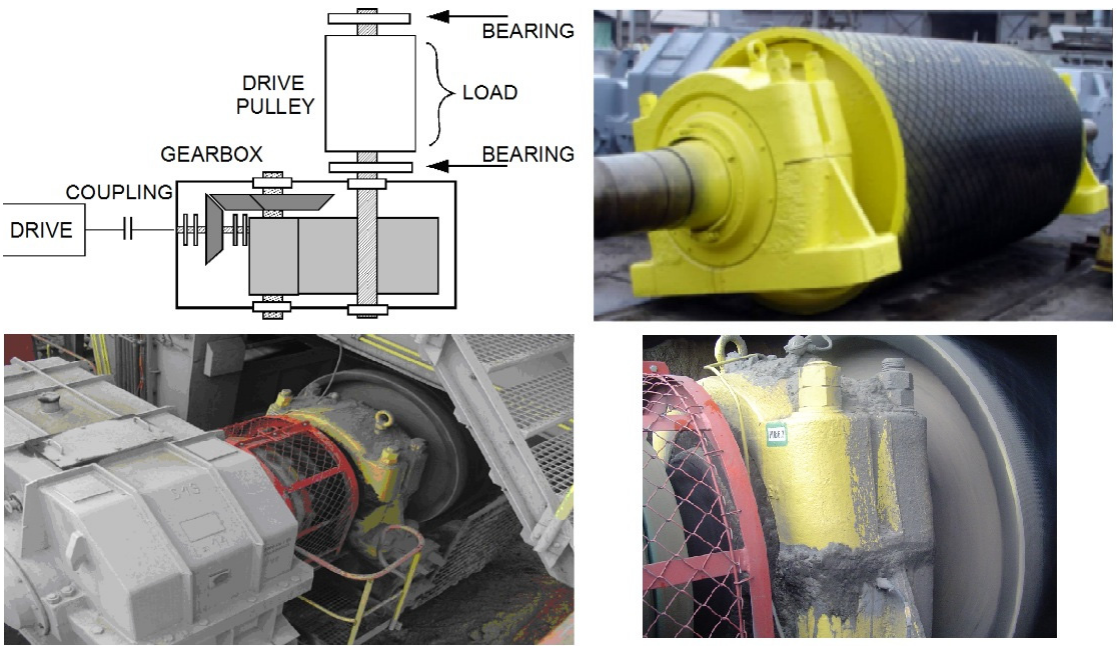
\includegraphics[width=0.68\textwidth]{wykresy/gb.PNG}
\caption{Object of interest}
\label{fig:gb}
\end{figure}

In this paper, authors analyze one-dimensional vibration signal acquired on rolling ball bearing of the drive pulley operating in belt conveyor driving station (see \ref{fig:gb}). Sampling frequency is equal to 19.2 kHz. Fig. \ref{fig:gb} presents the described gearbox and in Fig. \ref{fig:raw} time series of signal is presented. Signal is known to contain wideband impulses with modulation frequency 12.7 Hz corresponding to outer race local damage. More information can be found in other papers concerning the diagnostics of this machine \cite{zimroz2009some}. Kurtosis value for this sample is equal to 3.09.

\begin{figure}[ht!]
\centering
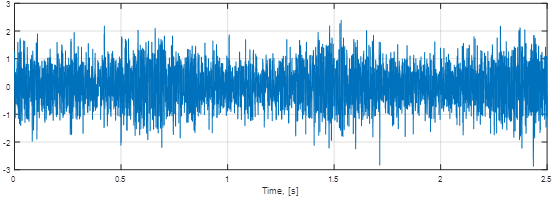
\includegraphics[width=0.68\textwidth]{wykresy/raw.png}
\caption{Raw input signal}
\label{fig:raw}
\end{figure}

\subsection{Evaluation of the algorithm performance on industrial data}



General results of the algorithm operation are presented in Fig. \ref{fig:real1}. One can see that input signal (Fig. \ref{fig:real1}a) processed with obtained filter reveals damage-related impulses in a very clear way, achieving kurtosis value of 87.23, which denotes the improvement by 2722$\%$ (Fig. \ref{fig:real1}d). Such high ratio (nearly 30 times the original value) can be the first indication of the presence of local damage. Envelope spectrum of input and output signal are presented in Fig. \ref{fig:real1}b and e respectively. Spectrograms of input and output signals (Fig. \ref{fig:real1}c and f respectively) present the time-frequency structure comparison between them and evaluate the obtained IFB. Magnitude response shows that optimization process created the filter that turn out to be arbitrarily custom and practically impossible to obtain by manual design (Fig. \ref{fig:real2}c). Phase linearity within passbands also has been achieved, which is essential for distortion avoidance (Fig. \ref{fig:real2}d). Vector of obtained filter coefficients is presented in Fig. \ref{fig:real2}a). 

\begin{figure}[ht!]
\centering
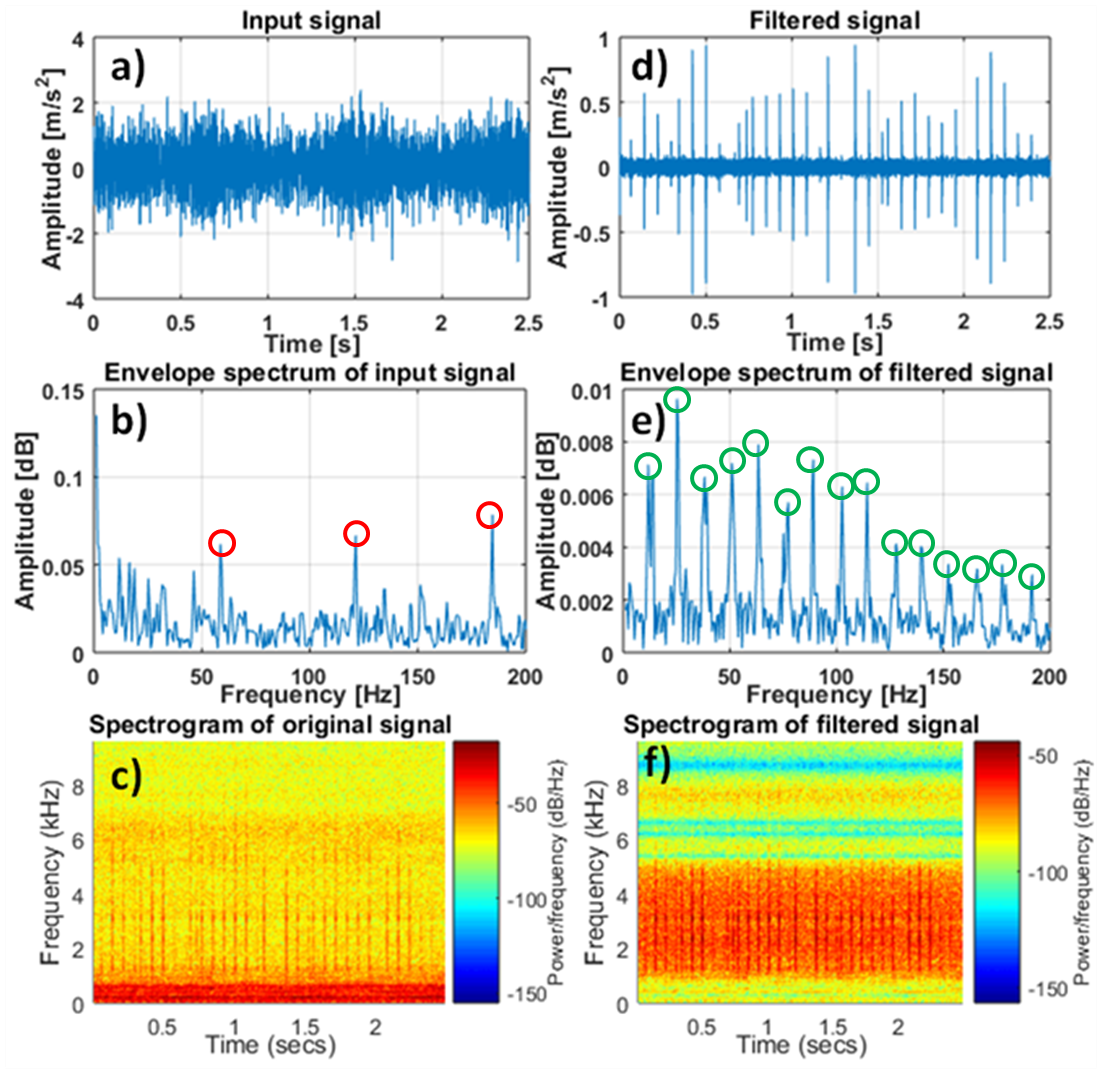
\includegraphics[width=0.8\textwidth]{wykresy/real1.png}
\caption{Comparison between real-life input and output signals describing damaged bearing: a) time series of input signal, d) time series of filtered signal, b) envelope spectrum of input signal (60 Hz component and its multiples are the harmonic frequencies of a power grid), e) envelope spectrum of output signal (12.7 Hz component and its multiples are related to damage of the bearing), c) spectrogram of input signal, f) spectrogram of output signal}
\label{fig:real1}
\end{figure}

Even brief visual inspection if the coefficients can provide information about some underlying low-cut character of the filter, which is very important for suppressing low-frequency high-energy components present in the input signal.

Fig. \ref{fig:real2}b) presents the progression of kurtosis value being the fitness function for the GA. Two main aspects of this curve can be distinguished:

\begin{itemize}
    \item jagged growth,
    \item points of decreasing value occurring occasionally throughout the whole process.
\end{itemize}

\begin{figure}[ht!]
\centering
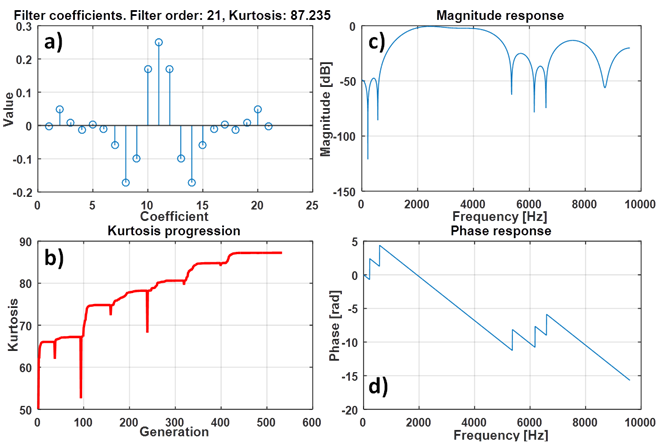
\includegraphics[width=0.8\textwidth]{wykresy/real2.png}
\caption{Final results of filter optimization for real-life damaged case: a) vector of filter coefficients, b) fitness progression, c) magnitude response of obtained filter, d) phase response of obtained filter}
\label{fig:real2}
\end{figure}

\begin{figure}[ht!]
\centering
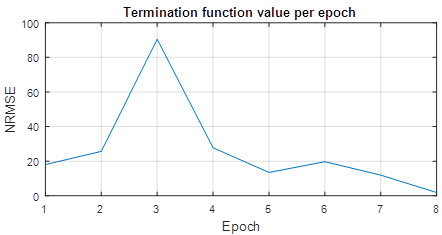
\includegraphics[width=0.8\textwidth]{wykresy/real3.png}
\caption{Values of termination function for real signal.}
\label{fig:real3}
\end{figure}

Jagged growth is the first inherent property of the progressiveness of GA. At the beginning filter is short and its fitness value is not expected to be very high. It improves within a single epoch, but not by far. In the next epoch filter becomes longer, which rapidly increases its capability to achieve better fitness. Extending filter length provides more progress than optimization within a single epoch, but for the reasons explained in \textcolor{red}{section} \ref{pga} this is essential for overall outcome and algorithm should not begin the operation with longer filter in the first place. Points of decreasing fitness value are another inherent property of GA progressiveness. This effect, every time it occurs, lasts only one generation being the consequence of filter prolonging operation. When new epoch begins, two additional coefficients are appended to the coefficient vector. Since those values are random, most of the time filter turns out to be worse than the last one from the previous epoch, and its fitness is lower. After that, in the next generation algorithm recognizes new possibilities and requires one or two generations to evolve the filter higher than ever before, continuing the overall optimization process. Termination function values are presented in Fig. \ref{fig:real3}. Final value that algorithm terminates at, is equal to 2.06, which is the first value of NRMSE that dropped below the 5$\%$ threshold.

\section{Discussion}

In machine diagnostics, obtaining decision about the technical condition of investigated machine is the end objective. In presented methodology one can observe strong correlation between kurtosis value after filtration and actual information about present damage. Hence, it is proposed to establish threshold of fitness value equal to 100$\%$ increase (200$\%$ of initial value). Results with fitness value lower than proposed level would be labeled as healthy, and higher – as damaged. In presented research damaged cases reached levels of nearly 3000$\%$ and nearly 400$\%$, and healthy case reached only 1$\%$ of increase.

\subsection{Comparison with classical methods}

One of the most recognized methods for IFB determination is filtration using filter determined by kurtogram. The kurtogram is a fourth-order spectral analysis tool elaborated for detecting and characterising nonstationarities in a signal. It relies on the assertion that each type of transient is associated with an optimal frequency/frequency resolution dyad (\textit{f}; $\delta$\textit{f}) which maximises the kurtosis \cite{antoni2007fast}.

Another method used for comparison is spectral kurtosis introduced by Antoni and Randall is regarded as one of the most powerful and popular approaches to localize informative frequency band, especially for vibration signal analysis \cite{randall2011rolling}. The general principle of operation is to calculate kurtosis value for each frequency bin of the spectrogram (\ref{eq:kurtosis}). As a result, one can obtain indicator of impulsiveness across the signal spectrum, which allows to determine which frequency bands carry the most visible information about the damage-related impulsive behavior. Vector of spectral kurtosis can be then used as a filter to extract those impulsive components from the signal.



% \begin{figure}[ht!]
% \centering
% 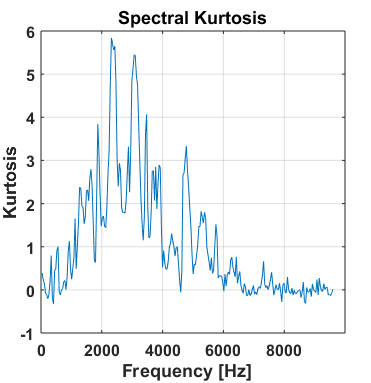
\includegraphics[width=0.9\textwidth]{wykresy/SK.png}
% \caption{Spectral Kurtosis function for real signal.}
% \label{fig:SK}
% \end{figure}


\begin{figure}[!ht]
  \centering
  \begin{subfigure}[b]{0.46\textwidth}
      \centering
     % \captionsetup{skip=0.01pt}
      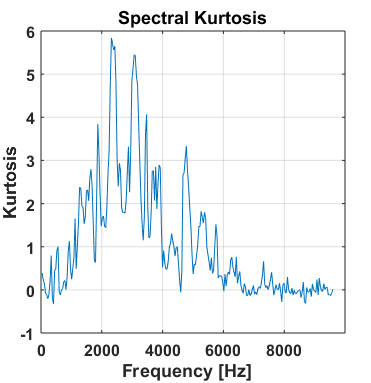
\includegraphics[width=\textwidth]{wykresy/SK}
      \caption{SK function for raw signal}
      \label{fig:SK}
  \end{subfigure}
  %\hfill
  \begin{subfigure}[b]{0.5\textwidth}
      \centering
    %  \captionsetup{skip=0.01pt}
		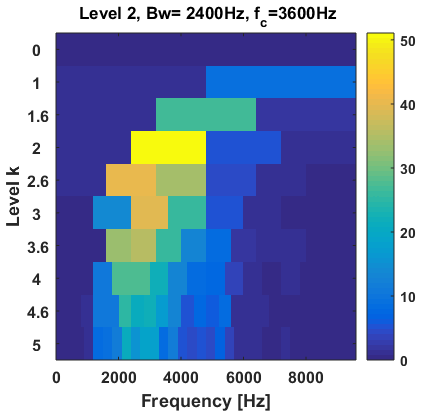
\includegraphics[width=\textwidth]{wykresy/kurtogram}
        \caption{Kurtogram of raw signal}
    \label{fig:kurtogram}
  \end{subfigure}
  \vspace{-5pt}
  \caption{Selectors used for comparison}
  \label{fig:comps}
\end{figure}


As a point of reference, authors compare the results to filtration based on SK and kurtogram for real industrial signal. It is important to mention at this point that for method comparison authors use envelopes because the way that kurtogram is calculated only allows to obtain envelope after filtration. Spectral kurtosis function for this data is presented in Fig. \ref{fig:SK}, and kurtogram in Fig. \ref{fig:kurtogram}. Envelopes of raw signal filtered with all three methods are presented in Fig. \ref{fig:comp}. In this comparison envelopes are used, since for the way that kurtogram filtering is implemented, only signal envelope is possible to be obtained. It can be easily seen that signal filtered with SK is characterized with much stronger noisefloor than after filtration with evolved filter or kurtogram-based filter. That causes weaker impulses to be lost in noise. Furthermore, kurtosis and Signal-to-Noise Ratio (SNR) values are also a lot lower than for presented method and kurtogram method.

% Initial signal (Envelope kurtosis=3,56) filtered with SK is characterized with envelope kurtosis value equal to 38, filtered with Kurtogram-based filter while after filtering with evolved filter kurtosis rises up to 87,23 (and even higher, if longer filter evolution were allowed).

\begin{table}[ht!]
    \centering
    \caption{Parameters of compared results}
  \begin{tabular}{|l|l|l|}
    \hline
    \textbf{Method} & \textbf{Envelope kurtosis} & \textbf{Envelope SNR [dBc]} \\ \hline
         Raw signal & 3,56 & -7,1 \\ \hline
         PGA-filtered & 129 & -14,02 \\ \hline
         Kurtogram-filtered & 51 & -13,93 \\ \hline
         SK-filtered & 38 & -9,9 \\
         
    \hline
    \end{tabular}
    \label{tab:tab3}
\end{table}

Another aspect worth noting is the rotational speed of the bearing. Presented method is based on the assumption that rotational speed is constant. Of course, authors realize that it is not, but the conditions of measurement of real signal allow to believe that machine was operating with quasi-constant speed for the given period of time. In addition, minor variations in rotational speed are not crucial for the performance of this method, but for large speed fluctuation, number of impulses might affect kurtosis and indeed it might lead to false results.

\begin{figure}[ht!]
\centering
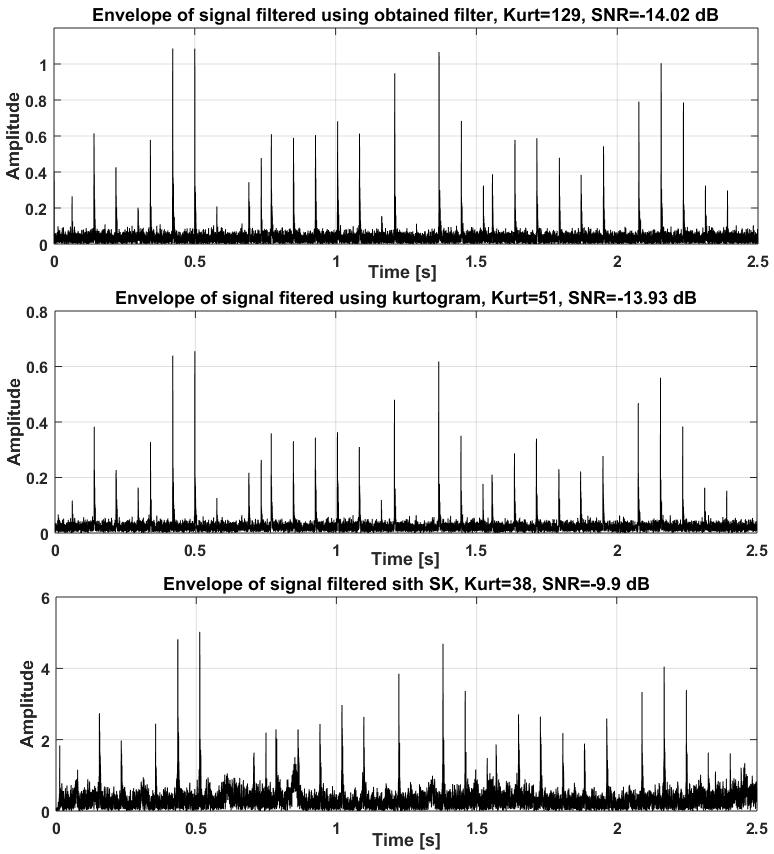
\includegraphics[width=0.8\textwidth]{wykresy/comp.png}
\caption{Comparison of envelopes of signals after filtration with PGA filter (top panel), using kurtogram (middle panel) and using spectral kurtosis (bottom panel)}
\label{fig:comp}
\end{figure}


\section{Conclusions}

In this paper we have introduced a new method of local damage detection based on genetic algorithm, applied to the real and simulated vibration signals. In opposition to using genetic algorithms for fine-tuning of designed filters or designing filters according to stated specification, it is proposed to design filter from scratch specifically for regarded input data. Filter construction is realized by evolving symmetric filter coefficient vector in order to obtain linear-phase FIR filter using odd amount of filter coefficients. Additionally, the aspect of progressiveness for genetic algorithm is proposed, which helps to better direct the evolution. Such approach makes the calculations faster and more efficient. Method is automatic, data-driven and requires no prior knowledge about the input signal. Termination criterion limits the computations only to necessary amount, and progressive construction of the algorithm provides robustness of avoiding misguided direction of evolution. Presented method has been compared with two classical methods for IFB determination, and the results are shown to be better in terms of kurtosis and SNR of output signals.

\section*{Acknowledgments}

The work of A.Michalak is supported by the Framework Programme for Research and Innovation Horizon 2020 under grant agreement n. 636834 (DISIRE - Integrated Process Control based on Distributed In-Situ Sensors into Raw Material and Energy Feedstock).

The work J.Wodecki and R.Zimroz is supported by the Statutory Grant no. 0401/0166/16

\section*{References}

\bibliography{mybibfile}

\end{document}